Como ya sabemos, al transmitir datos, el medio por el que viaja puede derivar en que los datos esten corruptos; esto debido a que el medio no es perfecto \\${ }$\\
Si enviaramos los datos tal cual, el problema sería que al llegar no habría nada que indique si esta mal, el receptor lo aceptaría y el usuario vería posiblemente la información erronea. Una forma de lidiar con esto es a traves de la redundancia (que sería esa información extra enviada que se utiliza para detectar el error). Una de estas es usando un bit de paridad, pero aún así, este método presenta limitaciones, ya que solo \textbf{funciona con un bit} de error, en este trabajo se veran algunos de estos métodos.
\subsection*{Checksum}
Es un método de código de bloque donde se crea una suma de verificación  basada en los valores de datos de los bloques que se transmiten y se agregarán a los datos. Cuando el receptor recibe los datos, se calcula la nueva suma y se compara con la existente.
\subsubsection*{Ejemplo}
\subsection*{Cyclic Redundancy Check (CRC)}
\subsection*{Código de Hamming}
 

 
%\begin{figure}[H]
%\centering
%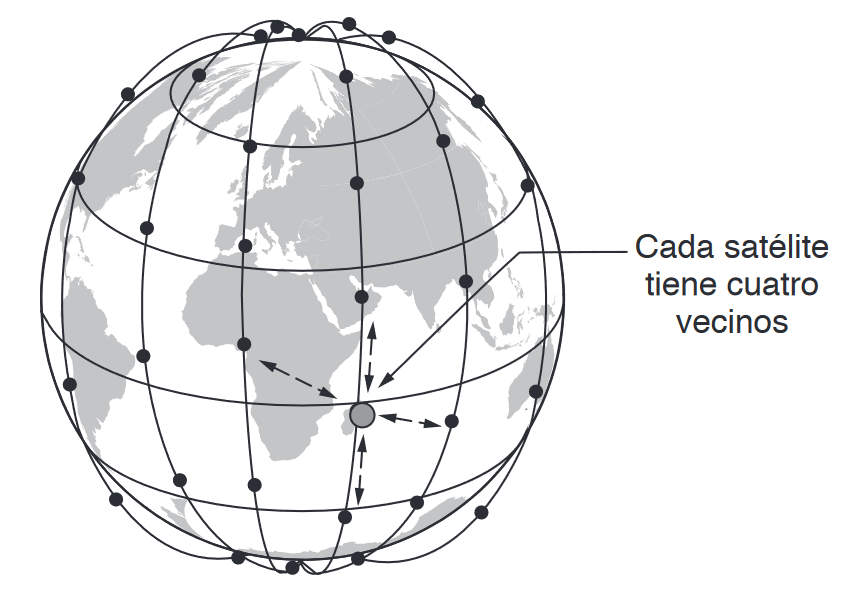
\includegraphics[page=1,scale=0.7]{SATELITES2.png}
%\caption{Satélites Iridium \textit{(Redes de Computadoras, Tanenbaum 4ta Edición, Pagina 105)}}
%\end{figure}

%\begin{figure}[H]
%\centering
%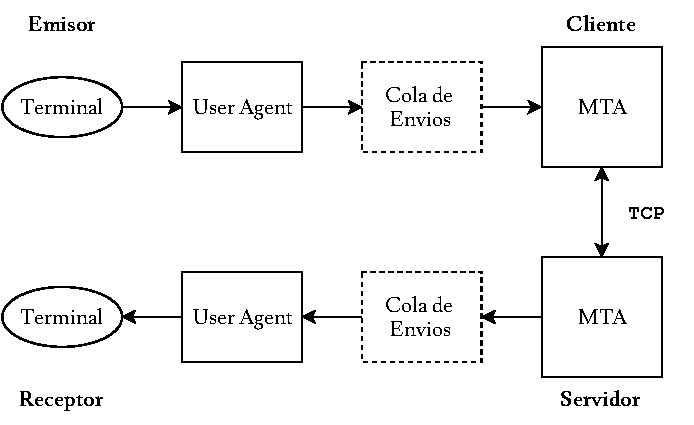
\includegraphics[page=1,scale=0.7]{SMTP.pdf}
%\caption{Esquema de funcionamiento de SMTP}
%\end{figure}
